\documentclass[tikz,convert={density=150,size=600,outext=.png}]{standalone}
\usetikzlibrary{shapes, calc, arrows, fit, positioning, decorations, patterns, decorations.pathreplacing, chains, snakes}

\begin{document}
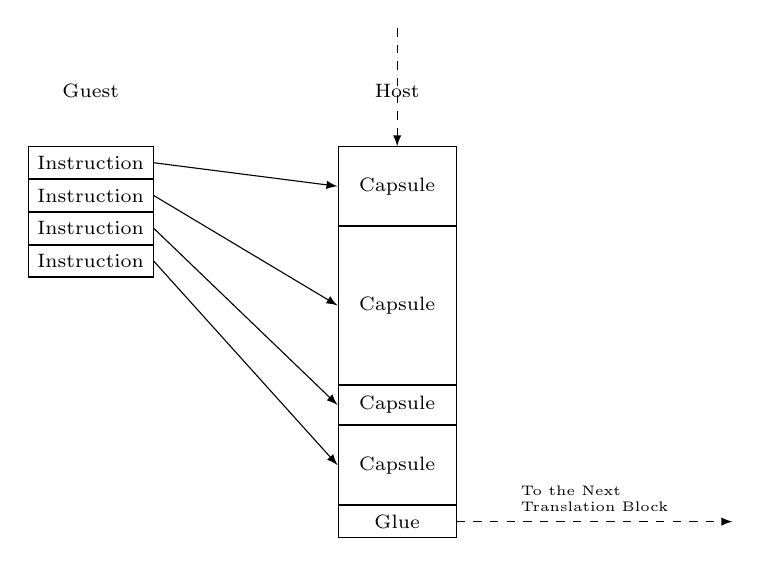
\begin{tikzpicture}[font=\scriptsize, >=latex]

\node (guest) {Guest};
\node[right=3cm of guest] (host) {Host};

\node[draw, minimum width = 0.7cm, below =0.5cm of guest] (gi1) {Instruction};
\node[draw, minimum width = 0.7cm, below = 0cm of gi1] (gi2) {Instruction};
\node[draw, minimum width = 0.7cm, below = 0cm of gi2] (gi3) {Instruction};
\node[draw, minimum width = 0.7cm, below = 0cm of gi3] (gi4) {Instruction};

\node[draw, minimum width = 1.5cm, minimum height = 1cm, below =0.5cm of host] (hi1) {Capsule};
\node[draw, minimum width = 1.5cm, minimum height = 2cm, below = 0cm of hi1] (hi2) {Capsule};
\node[draw, minimum width = 1.5cm, minimum height = 0.5cm, below = 0cm of hi2] (hi3) {Capsule};
\node[draw, minimum width = 1.5cm, minimum height = 1cm, below = 0cm of hi3] (hi4) {Capsule};
\node[draw, minimum width = 1.5cm, below = 0cm of hi4] (glue) {Glue};

\coordinate[right=3.5cm of glue] (next-block);
\coordinate[above=1.5cm of hi1] (entry);

\draw[->] (gi1.east) to (hi1.west);
\draw[->] (gi2.east) to (hi2.west);
\draw[->] (gi3.east) to (hi3.west);
\draw[->] (gi4.east) to (hi4.west);

\draw[->, dashed] (glue) -- (next-block) node[midway, above, font=\tiny, align=left] {To the Next\\Translation Block};
\draw[->, dashed] (entry) -- (hi1.north);

\end{tikzpicture}
\end{document}
